\usetikzlibrary{arrows.meta}
\usepackage{graphicx} %

\usepackage{bussproofs}
\def\figureRandFrame{

\begin{figure}
    \centering

\scriptsize{
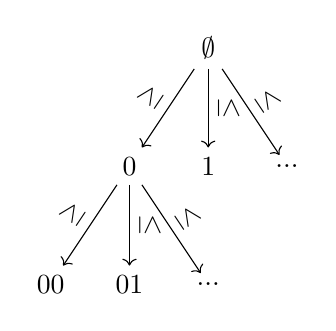
\begin{tikzpicture}
            % Root node
            \node (root) at (0,0) {$\emptyset$};
        
            % Second stage nodes
            \node (n1) at (-1,-1.5) {$0$};
            \node (n2) at (0,-1.5) {$1$};
            \node (n3) at (1,-1.5) {$...$};
        
            % Edges
            \draw[->] (root) -- (n1) node[midway, sloped, above] {$\geq$};
            \draw[->] (root) -- (n2) node[midway, sloped, above] {$\leq$};
            \draw[->] (root) -- (n3) node[midway, sloped, above] {$\leq$};
            
            % Third stage nodes
            \node (n00) at (-2,-3) {$00$};
            \node (n01) at (-1,-3) {$01$};
            \node (n02) at (0,-3) {$...$};
        
            % Edges
            \draw[->] (n1) -- (n00) node[midway, sloped, above] {$\geq$};
            \draw[->] (n1) -- (n01) node[midway, sloped, above] {$\leq$};
            \draw[->] (n1) -- (n02) node[midway, sloped, above] {$\leq$};
        
        \end{tikzpicture}
        \hspace{30pt}
        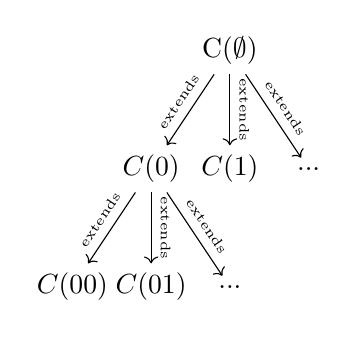
\begin{tikzpicture}
            % Root node
            \node (root) at (0,0) {C($\emptyset$)};
        
            % Second stage nodes
            \node (n1) at (-1,-1.5) {$C(0)$};
            \node (n2) at (0,-1.5) {$C(1)$};
            \node (n3) at (1,-1.5) {$...$};
        
            % Edges
            \draw[->] (root) -- (n1) node[midway, sloped, above] {\tiny{extends}};
            \draw[->] (root) -- (n2) node[midway, sloped, above] {\tiny{extends}};
            \draw[->] (root) -- (n3) node[midway, sloped, above] {\tiny{extends}};
            
            % Third stage nodes
            \node (n00) at (-2,-3) {$C(00)$};
            \node (n01) at (-1,-3) {$C(01)$};
            \node (n02) at (0,-3) {$...$};
        
            % Edges
            \draw[->] (n1) -- (n00) node[midway, sloped, above] {\tiny{extends}};
            \draw[->] (n1) -- (n01) node[midway, sloped, above] {\tiny{extends}};
            \draw[->] (n1) -- (n02) node[midway, sloped, above] {\tiny{extends}};

        \end{tikzpicture}
  

}

    \caption{R and a Kripke frame. }
    \label{fig:enter-label}
    
\end{figure}
}


\def\TableauxDevelopmentExampleFigure{
    
\begin{figure}
    \centering
    \makebox[\textwidth][c]{%
    \resizebox{0.95\textwidth}{!}{
    
    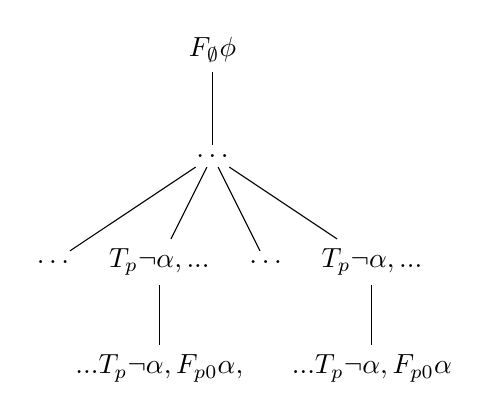
\begin{tikzpicture}[scale=0.9]
    \node {$F_{\emptyset}\phi$}
        child {node {$\ldots$}
            child {node {$\ldots$}}
            child {node {$T_{p} \neg \alpha, ...$}
                child {node {$ ... T_{p} \neg \alpha, F_{p0} \alpha,$}}}
            child {node {$\ldots$}}
            child {node {$T_{p} \neg \alpha, ...$}
                child {node {$ ... T_{p} \neg \alpha,F_{p0} \alpha$}}}};
    \end{tikzpicture}%
    
    
    
    \hspace{0.5cm} \raisebox{1.8cm}{$\hookleftarrow$} 
    \hspace{0.5cm}
    \raisebox{1.25cm}{
    \begin{tikzpicture}[scale=0.9]
    \node {$F_{\emptyset}\phi$}
        child {node {$\ldots$}
            child {node {$\ldots$}}
            child {node {$T_{p} \neg \alpha, ...$}}
            child {node {$\ldots$}}
            child {node {$T_{p} \neg \alpha, ...$}}};
    \end{tikzpicture}
    }
    %
    }%
    }
    \caption{Example of $\hookleftarrow(T \neg \alpha ,\tau)$ and $\tau$. } 
    \label{fig:tree_expansion}
    \end{figure}
}


\def\tableauxCumulativeAndNonCumulativeExampleFigureClassical{

        \centering
        \scriptsize{
        \makebox[\textwidth][c]{%
        \resizebox{1\textwidth}{!}{
        \begin{tikzpicture}
            % Root node
            \node (root) at (0,0) {$F \alpha \to \neg \neg \alpha$};
            
            % Second stage nodes
            \node (n1) at (0,-1.5) {$T \alpha$};
            \draw[->] (root) -- (n1);
            
            % Third stage nodes
            \node (n2) at (0,-3) {$F \neg \neg \alpha$};
            \draw[->] (n1) -- (n2);
            
            % Fourth stage nodes
            \node (n3) at (0,-4.5) {$T \neg \alpha$};
            \draw[->] (n2) -- (n3);

            
            % Fifth stage nodes
            \node (n4) at (0,-6) {$F \alpha$};
            \draw[->] (n3) -- (n4);

            \node (n5) at (0,-7.5) {$T \neg \alpha$};
            \draw[->] (n4) -- (n5);

            \node (n6) at (0,-8.5) {X};
            \draw[->] (n5) -- (n6);
        \end{tikzpicture}

        \hspace{1cm}

        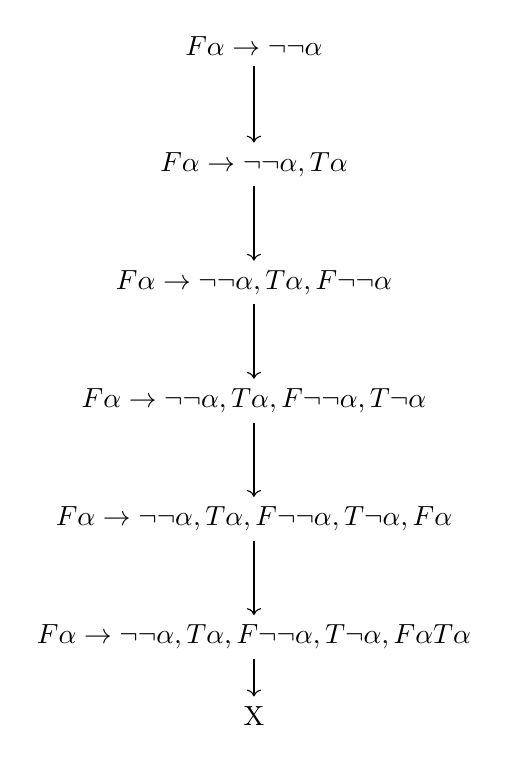
\begin{tikzpicture}
            % Root node
            \node (root) at (0,0) {$F \alpha \to \neg \neg \alpha$};
            
            % Second stage nodes
            \node (n1) at (0,-1.5) {$F \alpha \to \neg \neg \alpha, T \alpha$};
            \draw[->] (root) -- (n1);
            
            % Third stage nodes
            \node (n2) at (0,-3) {$F \alpha \to \neg \neg \alpha, T \alpha, F \neg \neg \alpha$};
            \draw[->] (n1) -- (n2);
            
            % Fourth stage nodes
            \node (n3) at (0,-4.5) {$F \alpha \to \neg \neg \alpha, T \alpha, F \neg \neg \alpha, T \neg \alpha$};
            \draw[->] (n2) -- (n3);
            
            % Fifth stage nodes
            \node (n4) at (0,-6) {$F \alpha \to \neg \neg \alpha, T \alpha, F \neg \neg \alpha, T \neg \alpha, F \alpha$};
            \draw[->] (n3) -- (n4);

            \node (n5) at (0,-7.5) {$F \alpha \to \neg \neg \alpha, T \alpha, F \neg \neg \alpha, T \neg \alpha, F \alpha T \alpha$};
            \draw[->] (n4) -- (n5);


            \node (n6) at (0,-8.5) {X};
            \draw[->] (n5) -- (n6);
        \end{tikzpicture}

        \hspace{1cm}

        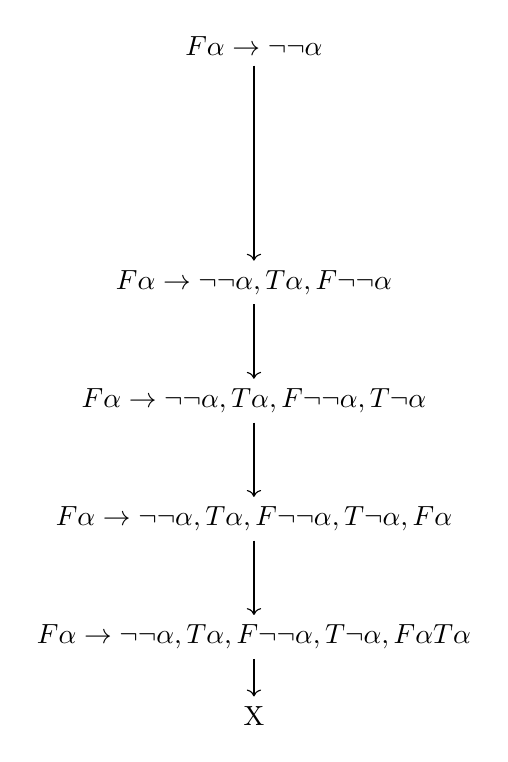
\begin{tikzpicture}
            % Root node
            \node (root) at (0,0) {$F \alpha \to \neg \neg \alpha$};
            
            % Second stage nodes
            
            % Third stage nodes
            \node (n2) at (0,-3) {$F \alpha \to \neg \neg \alpha, T \alpha, F \neg \neg \alpha$};
            \draw[->] (root) -- (n2);
            
            % Fourth stage nodes
            \node (n3) at (0,-4.5) {$F \alpha \to \neg \neg \alpha, T \alpha, F \neg \neg \alpha, T \neg \alpha$};
            \draw[->] (n2) -- (n3);
            
            % Fifth stage nodes
            \node (n4) at (0,-6) {$F \alpha \to \neg \neg \alpha, T \alpha, F \neg \neg \alpha, T \neg \alpha, F \alpha$};
            \draw[->] (n3) -- (n4);


            \node (n5) at (0,-7.5) {$F \alpha \to \neg \neg \alpha, T \alpha, F \neg \neg \alpha, T \neg \alpha, F \alpha T \alpha$};
            \draw[->] (n4) -- (n5);


            \node (n6) at (0,-8.5) {X};
            \draw[->] (n5) -- (n6);
        \end{tikzpicture}
        }
        }
    }
}




\def\tableauxClassicalExampleFigure{

        \centering
        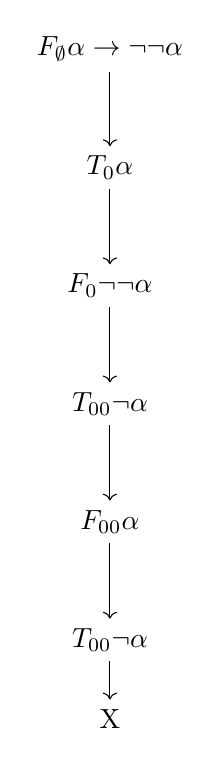
\begin{tikzpicture}
            % Root node
            \node (root) at (0,0) {$F_{\emptyset} \alpha \to \neg \neg \alpha$};
            
            % Second stage nodes
            \node (n1) at (0,-1.5) {$T_{0} \alpha$};
            \draw[->] (root) -- (n1);
            
            % Third stage nodes
            \node (n2) at (0,-3) {$F_{0} \neg \neg \alpha$};
            \draw[->] (n1) -- (n2);
            
            % Fourth stage nodes
            \node (n3) at (0,-4.5) {$T_{00} \neg \alpha$};
            \draw[->] (n2) -- (n3);

            
            % Fifth stage nodes
            \node (n4) at (0,-6) {$F_{00} \alpha$};
            \draw[->] (n3) -- (n4);

            \node (n5) at (0,-7.5) {$T_{00} \neg \alpha$};
            \draw[->] (n4) -- (n5);

            \node (n6) at (0,-8.5) {X};
            \draw[->] (n5) -- (n6);
        \end{tikzpicture}


        }





\def\tableauxCumulativeAndNonCumulativeExampleFigure{

        \centering
        \scriptsize{
        \makebox[\textwidth][c]{%
        \resizebox{1\textwidth}{!}{
        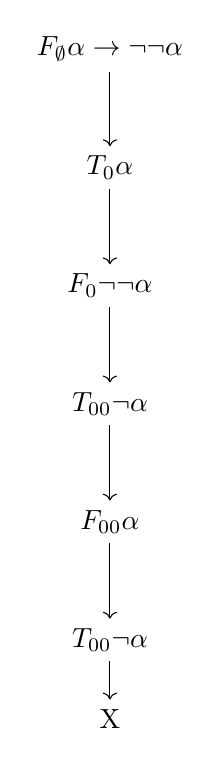
\begin{tikzpicture}
            % Root node
            \node (root) at (0,0) {$F_{\emptyset} \alpha \to \neg \neg \alpha$};
            
            % Second stage nodes
            \node (n1) at (0,-1.5) {$T_{0} \alpha$};
            \draw[->] (root) -- (n1);
            
            % Third stage nodes
            \node (n2) at (0,-3) {$F_{0} \neg \neg \alpha$};
            \draw[->] (n1) -- (n2);
            
            % Fourth stage nodes
            \node (n3) at (0,-4.5) {$T_{00} \neg \alpha$};
            \draw[->] (n2) -- (n3);

            
            % Fifth stage nodes
            \node (n4) at (0,-6) {$F_{00} \alpha$};
            \draw[->] (n3) -- (n4);

            \node (n5) at (0,-7.5) {$T_{00} \neg \alpha$};
            \draw[->] (n4) -- (n5);

            \node (n6) at (0,-8.5) {X};
            \draw[->] (n5) -- (n6);
        \end{tikzpicture}

        \hspace{1cm}

        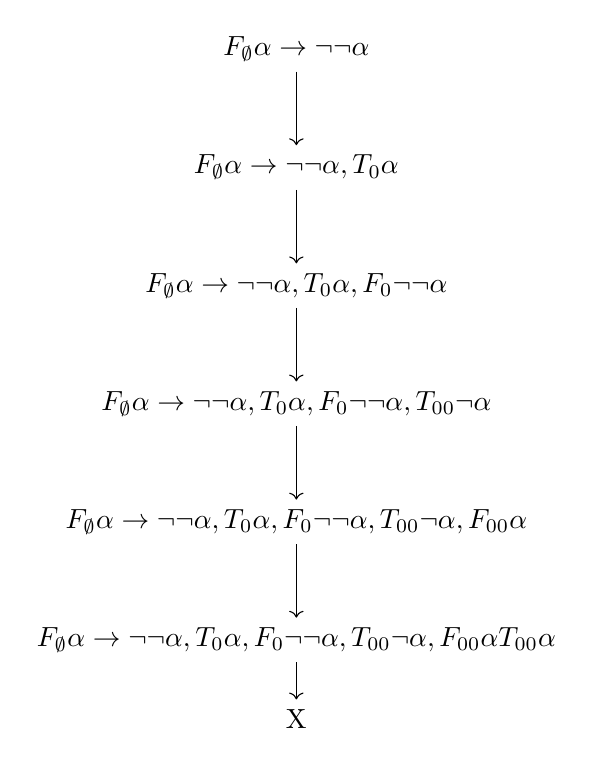
\begin{tikzpicture}
            % Root node
            \node (root) at (0,0) {$F_{\emptyset} \alpha \to \neg \neg \alpha$};
            
            % Second stage nodes
            \node (n1) at (0,-1.5) {$F_{\emptyset} \alpha \to \neg \neg \alpha, T_{0} \alpha$};
            \draw[->] (root) -- (n1);
            
            % Third stage nodes
            \node (n2) at (0,-3) {$F_{\emptyset} \alpha \to \neg \neg \alpha, T_{0} \alpha, F_{0} \neg \neg \alpha$};
            \draw[->] (n1) -- (n2);
            
            % Fourth stage nodes
            \node (n3) at (0,-4.5) {$F_{\emptyset} \alpha \to \neg \neg \alpha, T_{0} \alpha, F_{0} \neg \neg \alpha, T_{00} \neg \alpha$};
            \draw[->] (n2) -- (n3);
            
            % Fifth stage nodes
            \node (n4) at (0,-6) {$F_{\emptyset} \alpha \to \neg \neg \alpha, T_{0} \alpha, F_{0} \neg \neg \alpha, T_{00} \neg \alpha, F_{00} \alpha$};
            \draw[->] (n3) -- (n4);

            \node (n5) at (0,-7.5) {$F_{\emptyset} \alpha \to \neg \neg \alpha, T_{0} \alpha, F_{0} \neg \neg \alpha, T_{00} \neg \alpha, F_{00} \alpha T_{00} \alpha$};
            \draw[->] (n4) -- (n5);


            \node (n6) at (0,-8.5) {X};
            \draw[->] (n5) -- (n6);
        \end{tikzpicture}

        \hspace{1cm}

        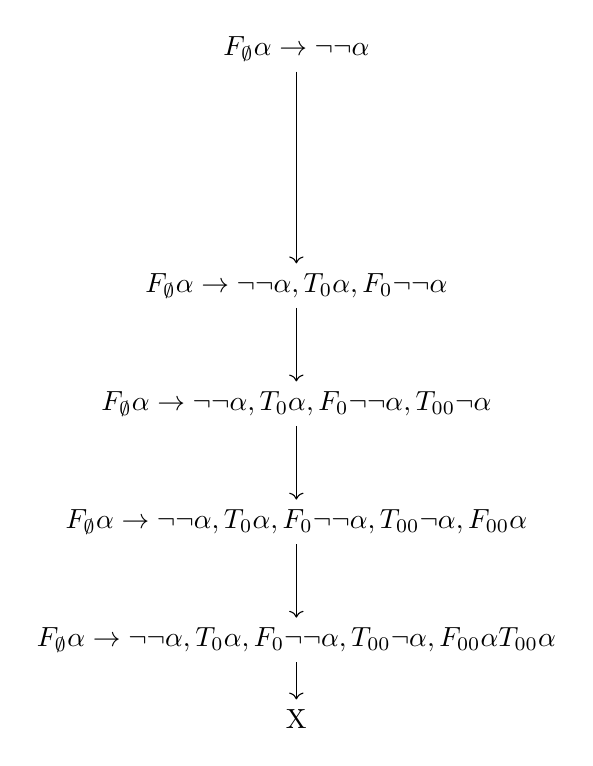
\begin{tikzpicture}
            % Root node
            \node (root) at (0,0) {$F_{\emptyset} \alpha \to \neg \neg \alpha$};
            
            % Second stage nodes
            
            % Third stage nodes
            \node (n2) at (0,-3) {$F_{\emptyset} \alpha \to \neg \neg \alpha, T_{0} \alpha, F_{0} \neg \neg \alpha$};
            \draw[->] (root) -- (n2);
            
            % Fourth stage nodes
            \node (n3) at (0,-4.5) {$F_{\emptyset} \alpha \to \neg \neg \alpha, T_{0} \alpha, F_{0} \neg \neg \alpha, T_{00} \neg \alpha$};
            \draw[->] (n2) -- (n3);
            
            % Fifth stage nodes
            \node (n4) at (0,-6) {$F_{\emptyset} \alpha \to \neg \neg \alpha, T_{0} \alpha, F_{0} \neg \neg \alpha, T_{00} \neg \alpha, F_{00} \alpha$};
            \draw[->] (n3) -- (n4);


            \node (n5) at (0,-7.5) {$F_{\emptyset} \alpha \to \neg \neg \alpha, T_{0} \alpha, F_{0} \neg \neg \alpha, T_{00} \neg \alpha, F_{00} \alpha T_{00} \alpha$};
            \draw[->] (n4) -- (n5);


            \node (n6) at (0,-8.5) {X};
            \draw[->] (n5) -- (n6);
        \end{tikzpicture}
        }
        }
        }

}








\def\RulesIntuitionisticSequentCalculus{


\begin{table}[h!]
    \caption{Rules for intuitionistic multi-consequence sequent calculus.}\label{tab:intuitionistic}
\centering
\renewcommand{\arraystretch}{3} % Adjust row height
\begin{tabular}{|c|c|}  
\hline
\textbf{Rule} & \textbf{Inference} \\ \hline
Axiom  & $\AxiomC{}\UnaryInfC{$\alpha \vdash \alpha$}\DisplayProof$ \\ \hline
Weakening & $ \AxiomC{$\Gamma \vdash \Delta$}\UnaryInfC{$\Gamma, \alpha \vdash \Delta$}\DisplayProof$ \quad
$\AxiomC{$\Gamma \vdash \Delta$}\UnaryInfC{$\Gamma \vdash \Delta, \alpha$}\DisplayProof$ \\ \hline
Negation & 
$\RightLabel{\scriptsize{$\neg$L  $\neg \alpha$}}\AxiomC{$\Gamma , \vdash \alpha, \Delta$}\UnaryInfC{$\Gamma, \neg \alpha \vdash \Delta$}\DisplayProof$ \quad
$\RightLabel{\scriptsize{$\neg$R  $\neg \alpha$}}\AxiomC{$\Gamma, \alpha \vdash \color{white}{\Delta} $}\UnaryInfC{$\Gamma \vdash \neg \alpha, \color{white}{\Delta}$}\DisplayProof$ \\ \hline
Conjunction & 
$\RightLabel{\scriptsize{$\land$L  $\alpha \land \beta$}}\AxiomC{$\Gamma, \alpha, \beta \vdash \Delta$}\UnaryInfC{$\Gamma, \alpha \land \beta \vdash \Delta$}\DisplayProof$ \quad
$\RightLabel{\scriptsize{$\land$R $\alpha \land \beta$}}\AxiomC{$\Gamma \vdash \alpha, \Delta$}\AxiomC{$\Gamma \vdash \beta, \Delta$}\BinaryInfC{$\Gamma \vdash \alpha \land \beta, \Delta$}\DisplayProof$ \\ \hline
Disjunction & 
$\RightLabel{\scriptsize{$\lor$ L  $\alpha \lor \beta$}}\AxiomC{$\Gamma, \alpha \vdash \Delta$}\AxiomC{$\Gamma, \beta \vdash \Delta$}\BinaryInfC{$\Gamma, \alpha \lor \beta \vdash \Delta$}\DisplayProof$ \quad
$\RightLabel{\scriptsize{$\lor$ $R_{1}$  $\alpha \lor \beta$}}\AxiomC{$\Gamma \vdash \alpha, \Delta$}\UnaryInfC{$\Gamma \vdash \alpha \lor \beta, \Delta$}\DisplayProof$ \quad
$\RightLabel{\scriptsize{$\lor$ $R_{2}$ $\alpha \lor \beta$}}\AxiomC{$\Gamma \vdash \beta, \Delta$}\UnaryInfC{$\Gamma \vdash \alpha \lor \beta, \Delta$}\DisplayProof$ \\ \hline
Implication & 
$\RightLabel{\scriptsize{$\to$ L  $\alpha \to \beta$}}\AxiomC{$\Gamma \vdash \alpha, \Delta$}\AxiomC{$\Gamma, \beta \vdash \Delta$}\BinaryInfC{$\Gamma, \alpha \to \beta \vdash \Delta$}\DisplayProof$ \quad
$\RightLabel{\scriptsize{$\to$ R  $\alpha \to \beta$}}\AxiomC{$\Gamma, \alpha \vdash \beta$}\UnaryInfC{$\Gamma \vdash \alpha \to \beta$}\DisplayProof$ \\ \hline
Quantifiers & 
$\RightLabel{\scriptsize{$\forall$ L $\forall x \alpha(x)$}}\AxiomC{$\Gamma, \alpha(t) \vdash \Delta$}\UnaryInfC{$\Gamma, \forall x \alpha(x) \vdash \Delta$}\DisplayProof$ \quad
$\RightLabel{\scriptsize{$\forall$ R $\forall x \alpha(x)$}}\AxiomC{$\Gamma \vdash \alpha(y)$}\UnaryInfC{$\Gamma \vdash \forall x \alpha(x)$}\DisplayProof$ with y fresh \\ 
& 
$\RightLabel{\scriptsize{$\exists$ L $\exists x \alpha(x)$}}\AxiomC{$\Gamma, \alpha(y) \vdash \Delta$}\UnaryInfC{$\Gamma, \exists x \alpha(x) \vdash \Delta$}\DisplayProof$ with y fresh \quad
$\RightLabel{\scriptsize{$\exists$ R $\exists x \alpha(x)$}}\AxiomC{$\Gamma \vdash \alpha(t), \Delta$}\UnaryInfC{$\Gamma \vdash \exists x \alpha(x), \Delta$}\DisplayProof$ \\ \hline
Contraction & 
$\AxiomC{$\Gamma, \alpha, \alpha \vdash \Delta$}\UnaryInfC{$\Gamma, \alpha \vdash \Delta$}\DisplayProof$ \quad
$\AxiomC{$\Gamma \vdash \alpha, \alpha, \Delta$}\UnaryInfC{$\Gamma \vdash \alpha, \Delta$}\DisplayProof$ \\ \hline
\end{tabular}
\end{table}
}




\def\RulesIntuitionisticSequentCalculusSmall{

    \begin{table}[h!]
        \centering
    \renewcommand{\arraystretch}{3} % Adjust row height
     \begin{tabular}{cc}  
        $\RightLabel{Ax $\alpha$}\AxiomC{}\UnaryInfC{$\Gamma , \alpha \vdash \alpha,  \Delta$}\DisplayProof$ \\ 
        $ \AxiomC{$\Gamma \vdash \Delta$}\UnaryInfC{$\Gamma, \alpha \vdash \Delta$}\DisplayProof$ \quad
        $\AxiomC{$\Gamma \vdash \Delta$}\UnaryInfC{$\Gamma \vdash \Delta, \alpha$}\DisplayProof$ \\ 
        $\RightLabel{$\neg$L  $\neg \alpha$}\AxiomC{$\Gamma , \vdash \alpha, \Delta$}\UnaryInfC{$\Gamma, \neg \alpha \vdash \Delta$}\DisplayProof$ \quad
        $\RightLabel{$\neg$R  $\neg \alpha$}\AxiomC{$\Gamma, \alpha \vdash \color{white}{\Delta}$}\UnaryInfC{$\Gamma \vdash \neg \alpha \color{white}{,\Delta}$}\DisplayProof$ \\ 
        $\RightLabel{$\land$L  $\alpha \land \beta$}\AxiomC{$\Gamma, \alpha, \beta \vdash \Delta$}\UnaryInfC{$\Gamma, \alpha \land \beta \vdash \Delta$}\DisplayProof$ \quad
        $\RightLabel{$\land$R $\alpha \land \beta$}\AxiomC{$\Gamma \vdash \alpha, \Delta$}\AxiomC{$\Gamma \vdash \beta, \Delta$}\BinaryInfC{$\Gamma \vdash \alpha \land \beta, \Delta$}\DisplayProof$ \\ 
        $\RightLabel{$\lor$ L  $\alpha \lor \beta$}\AxiomC{$\Gamma, \alpha \vdash \Delta$}\AxiomC{$\Gamma, \beta \vdash \Delta$}\BinaryInfC{$\Gamma, \alpha \lor \beta \vdash \Delta$}\DisplayProof$ \quad
        $\RightLabel{$\lor$ R  $\alpha \lor \beta$}\AxiomC{$\Gamma \vdash \alpha,\beta \Delta$}\UnaryInfC{$\Gamma \vdash \alpha \lor \beta, \Delta$}\DisplayProof$ \\
        $\RightLabel{$\to$ L  $\alpha \to \beta$}\AxiomC{$\Gamma \vdash \alpha, \Delta$}\AxiomC{$\Gamma, \beta \vdash \Delta$}\BinaryInfC{$\Gamma, \alpha \to \beta \vdash \Delta$}\DisplayProof$ \quad
        $\RightLabel{$\to$ R  $\alpha \to \beta$}\AxiomC{$\Gamma, \alpha \vdash \beta \color{white}{, \Delta}$}\UnaryInfC{$\Gamma \vdash \alpha \to \beta\color{white}{,\Delta}$}\DisplayProof$ \\ 
        $\RightLabel{$\forall$ L $\forall x \alpha(x)$}\AxiomC{$\Gamma, \alpha(t) \vdash \Delta$}\UnaryInfC{$\Gamma, \forall x \alpha(x) \vdash \Delta$}\DisplayProof$ \quad
        $\RightLabel{$\forall$ R $\forall x \alpha(x)$}\AxiomC{$\Gamma \vdash \alpha(y) \color{white}{, \Delta}$}\UnaryInfC{$\Gamma \vdash \forall x \alpha(x) \color{white}{,\Delta}$}\DisplayProof$ \\ 
        $\RightLabel{$\exists$ L $\exists x \alpha(x)$}\AxiomC{$\Gamma, \alpha(y) \vdash \Delta$}\UnaryInfC{$\Gamma, \exists x \alpha(x) \vdash \Delta$}\DisplayProof$ \quad
        $\RightLabel{$\exists$ R $\exists x \alpha(x)$}\AxiomC{$\Gamma \vdash \alpha(t), \Delta$}\UnaryInfC{$\Gamma \vdash \exists x \alpha(x), \Delta$}\DisplayProof$ \\ 
        $\AxiomC{$\Gamma, \alpha, \alpha \vdash \Delta$}\UnaryInfC{$\Gamma, \alpha \vdash \Delta$}\DisplayProof$ \quad
        $\AxiomC{$\Gamma \vdash \alpha, \alpha, \Delta$}\UnaryInfC{$\Gamma \vdash \alpha, \Delta$}\DisplayProof$ \\ 
        \end{tabular}
    \end{table}
}

\def\RulesClassicalSequentCalculusSmall{

    \begin{table}[h!]
        \centering
    \renewcommand{\arraystretch}{3} % Adjust row height
     \begin{tabular}{cc}  
        $\RightLabel{Ax $\alpha$}\AxiomC{}\UnaryInfC{$\Gamma , \alpha \vdash \alpha,  \Delta$}\DisplayProof$ \\ 
        $ \AxiomC{$\Gamma \vdash \Delta$}\UnaryInfC{$\Gamma, \alpha \vdash \Delta$}\DisplayProof$ \quad
        $\AxiomC{$\Gamma \vdash \Delta$}\UnaryInfC{$\Gamma \vdash \Delta, \alpha$}\DisplayProof$ \\ 
        $\RightLabel{$\neg$L  $\neg \alpha$}\AxiomC{$\Gamma , \vdash \alpha, \Delta$}\UnaryInfC{$\Gamma, \neg \alpha \vdash \Delta$}\DisplayProof$ \quad
        $\RightLabel{$\neg$R  $\neg \alpha$}\AxiomC{$\Gamma, \alpha \vdash \Delta$}\UnaryInfC{$\Gamma \vdash \neg \alpha, \Delta$}\DisplayProof$ \\ 
        $\RightLabel{$\land$L  $\alpha \land \beta$}\AxiomC{$\Gamma, \alpha, \beta \vdash \Delta$}\UnaryInfC{$\Gamma, \alpha \land \beta \vdash \Delta$}\DisplayProof$ \quad
        $\RightLabel{$\land$R $\alpha \land \beta$}\AxiomC{$\Gamma \vdash \alpha, \Delta$}\AxiomC{$\Gamma \vdash \beta, \Delta$}\BinaryInfC{$\Gamma \vdash \alpha \land \beta, \Delta$}\DisplayProof$ \\ 
        $\RightLabel{$\lor$ L  $\alpha \lor \beta$}\AxiomC{$\Gamma, \alpha \vdash \Delta$}\AxiomC{$\Gamma, \beta \vdash \Delta$}\BinaryInfC{$\Gamma, \alpha \lor \beta \vdash \Delta$}\DisplayProof$ \quad
        $\RightLabel{$\lor$ R  $\alpha \lor \beta$}\AxiomC{$\Gamma \vdash \alpha, \beta \Delta$}\UnaryInfC{$\Gamma \vdash \alpha \lor \beta, \Delta$}\DisplayProof$ \\ 
        $\RightLabel{$\to$ L  $\alpha \to \beta$}\AxiomC{$\Gamma \vdash \alpha, \Delta$}\AxiomC{$\Gamma, \beta \vdash \Delta$}\BinaryInfC{$\Gamma, \alpha \to \beta \vdash \Delta$}\DisplayProof$ \quad
        $\RightLabel{$\to$ R  $\alpha \to \beta$}\AxiomC{$\Gamma, \alpha \vdash \beta, \Delta$}\UnaryInfC{$\Gamma \vdash \alpha \to \beta, \Delta$}\DisplayProof$ \\ 
        $\RightLabel{$\forall$ L $\forall x \alpha(x)$}\AxiomC{$\Gamma, \alpha(t) \vdash \Delta$}\UnaryInfC{$\Gamma, \forall x \alpha(x) \vdash \Delta$}\DisplayProof$ \quad
        $\RightLabel{$\forall$ R $\forall x \alpha(x)$}\AxiomC{$\Gamma \vdash \alpha(y), \Delta$}\UnaryInfC{$\Gamma \vdash \forall x \alpha(x), \Delta$}\DisplayProof$ \\ 
        $\RightLabel{$\exists$ L $\exists x \alpha(x)$}\AxiomC{$\Gamma, \alpha(y) \vdash \Delta$}\UnaryInfC{$\Gamma, \exists x \alpha(x) \vdash \Delta$}\DisplayProof$ \quad
        $\RightLabel{$\exists$ R $\exists x \alpha(x)$}\AxiomC{$\Gamma \vdash \alpha(t), \Delta$}\UnaryInfC{$\Gamma \vdash \exists x \alpha(x), \Delta$}\DisplayProof$ \\ 
        $\AxiomC{$\Gamma, \alpha, \alpha \vdash \Delta$}\UnaryInfC{$\Gamma, \alpha \vdash \Delta$}\DisplayProof$ \quad
        $\AxiomC{$\Gamma \vdash \alpha, \alpha, \Delta$}\UnaryInfC{$\Gamma \vdash \alpha, \Delta$}\DisplayProof$ \\ 
        \end{tabular}
    \end{table}
}


\def\RulesClassicalSequentCalculusSmallBF{
    \textcolor{black!30}{
        \tiny{
    \begin{table}[h!]
        \centering
    \renewcommand{\arraystretch}{3} % Adjust row height
     \begin{tabular}{cc}  
        \textcolor{black}{\boldmath{$\RightLabel{Ax $\alpha$}\AxiomC{}\UnaryInfC{$\Gamma , \alpha \vdash \alpha,  \Delta$}\DisplayProof$ }}\\ 
        $ \AxiomC{$\Gamma \vdash \Delta$}\UnaryInfC{$\Gamma, \alpha \vdash \Delta$}\DisplayProof$ \quad
        $\AxiomC{$\Gamma \vdash \Delta$}\UnaryInfC{$\Gamma \vdash \Delta, \alpha$}\DisplayProof$ \\ 
        $\RightLabel{$\neg$L  $\neg \alpha$}\AxiomC{$\Gamma , \vdash \alpha, \Delta$}\UnaryInfC{$\Gamma, \neg \alpha \vdash \Delta$}\DisplayProof$ \quad
        \textcolor{black}{\boldmath{$\RightLabel{$\neg$R  $\neg \alpha$}\AxiomC{$\Gamma, \alpha \vdash \Delta$}\UnaryInfC{$\Gamma \vdash \neg \alpha, \Delta$}\DisplayProof$}} \\ 
        $\RightLabel{$\land$L  $\alpha \land \beta$}\AxiomC{$\Gamma, \alpha, \beta \vdash \Delta$}\UnaryInfC{$\Gamma, \alpha \land \beta \vdash \Delta$}\DisplayProof$ \quad
        $\RightLabel{$\land$R $\alpha \land \beta$}\AxiomC{$\Gamma \vdash \alpha, \Delta$}\AxiomC{$\Gamma \vdash \beta, \Delta$}\BinaryInfC{$\Gamma \vdash \alpha \land \beta, \Delta$}\DisplayProof$ \\ 
        $\RightLabel{$\lor$ L  $\alpha \lor \beta$}\AxiomC{$\Gamma, \alpha \vdash \Delta$}\AxiomC{$\Gamma, \beta \vdash \Delta$}\BinaryInfC{$\Gamma, \alpha \lor \beta \vdash \Delta$}\DisplayProof$ \quad
        \textcolor{black}{\boldmath{$\RightLabel{$\lor$ R  $\alpha \lor \beta$}\AxiomC{$\Gamma \vdash \alpha, \beta ,\Delta$}\UnaryInfC{$\Gamma \vdash \alpha \lor \beta, \Delta$}\DisplayProof$}} \\ 
        $\RightLabel{$\to$ L  $\alpha \to \beta$}\AxiomC{$\Gamma \vdash \alpha, \Delta$}\AxiomC{$\Gamma, \beta \vdash \Delta$}\BinaryInfC{$\Gamma, \alpha \to \beta \vdash \Delta$}\DisplayProof$ \quad
        $\RightLabel{$\to$ R  $\alpha \to \beta$}\AxiomC{$\Gamma, \alpha \vdash \beta, \Delta$}\UnaryInfC{$\Gamma \vdash \alpha \to \beta, \Delta$}\DisplayProof$ \\ 
        $\RightLabel{$\forall$ L $\forall x \alpha(x)$}\AxiomC{$\Gamma, \alpha(t) \vdash \Delta$}\UnaryInfC{$\Gamma, \forall x \alpha(x) \vdash \Delta$}\DisplayProof$ \quad
        $\RightLabel{$\forall$ R $\forall x \alpha(x)$}\AxiomC{$\Gamma \vdash \alpha(y), \Delta$}\UnaryInfC{$\Gamma \vdash \forall x \alpha(x), \Delta$}\DisplayProof$ \\ 
        $\RightLabel{$\exists$ L $\exists x \alpha(x)$}\AxiomC{$\Gamma, \alpha(y) \vdash \Delta$}\UnaryInfC{$\Gamma, \exists x \alpha(x) \vdash \Delta$}\DisplayProof$ \quad
        $\RightLabel{$\exists$ R $\exists x \alpha(x)$}\AxiomC{$\Gamma \vdash \alpha(t), \Delta$}\UnaryInfC{$\Gamma \vdash \exists x \alpha(x), \Delta$}\DisplayProof$ \\ 
        $\AxiomC{$\Gamma, \alpha, \alpha \vdash \Delta$}\UnaryInfC{$\Gamma, \alpha \vdash \Delta$}\DisplayProof$ \quad
        $\AxiomC{$\Gamma \vdash \alpha, \alpha, \Delta$}\UnaryInfC{$\Gamma \vdash \alpha, \Delta$}\DisplayProof$ \\ 
        \end{tabular}
    \end{table}
        }
    }
}


\def\RulesIntuitionisticSequentCalculusSmallBF{
    \textcolor{black!30}{
        \tiny{
    \begin{table}[h!]
        \centering
    \renewcommand{\arraystretch}{3} % Adjust row height
     \begin{tabular}{cc}  
        \textcolor{black}{\boldmath{$\RightLabel{Ax $\alpha$}\AxiomC{}\UnaryInfC{$\Gamma , \alpha \vdash \alpha,  \Delta$}\DisplayProof$}} \\ 
        $ \AxiomC{$\Gamma \vdash \Delta$}\UnaryInfC{$\Gamma, \alpha \vdash \Delta$}\DisplayProof$ \quad
        $\AxiomC{$\Gamma \vdash \Delta$}\UnaryInfC{$\Gamma \vdash \Delta, \alpha$}\DisplayProof$ \\ 
        $\RightLabel{$\neg$L  $\neg \alpha$}\AxiomC{$\Gamma , \vdash \alpha, \Delta$}\UnaryInfC{$\Gamma, \neg \alpha \vdash \Delta$}\DisplayProof$ \quad
        \textcolor{black}{\boldmath{$\RightLabel{$\neg$R  $\neg \alpha$}\AxiomC{$\Gamma, \alpha \vdash \color{white}{\Delta}$}\UnaryInfC{$\Gamma \vdash \neg \alpha \color{white}{,\Delta}$}\DisplayProof$}} \\ 
        $\RightLabel{$\land$L  $\alpha \land \beta$}\AxiomC{$\Gamma, \alpha, \beta \vdash \Delta$}\UnaryInfC{$\Gamma, \alpha \land \beta \vdash \Delta$}\DisplayProof$ \quad
        $\RightLabel{$\land$R $\alpha \land \beta$}\AxiomC{$\Gamma \vdash \alpha, \Delta$}\AxiomC{$\Gamma \vdash \beta, \Delta$}\BinaryInfC{$\Gamma \vdash \alpha \land \beta, \Delta$}\DisplayProof$ \\ 
        $\RightLabel{$\lor$ L  $\alpha \lor \beta$}\AxiomC{$\Gamma, \alpha \vdash \Delta$}\AxiomC{$\Gamma, \beta \vdash \Delta$}\BinaryInfC{$\Gamma, \alpha \lor \beta \vdash \Delta$}\DisplayProof$ \quad
        \textcolor{black}{\boldmath{$\RightLabel{$\lor$ R  $\alpha \lor \beta$}\AxiomC{$\Gamma \vdash \alpha,\beta, \Delta$}\UnaryInfC{$\Gamma \vdash \alpha \lor \beta, \Delta$}\DisplayProof$}} \\
        $\RightLabel{$\to$ L  $\alpha \to \beta$}\AxiomC{$\Gamma \vdash \alpha, \Delta$}\AxiomC{$\Gamma, \beta \vdash \Delta$}\BinaryInfC{$\Gamma, \alpha \to \beta \vdash \Delta$}\DisplayProof$ \quad
        $\RightLabel{$\to$ R  $\alpha \to \beta$}\AxiomC{$\Gamma, \alpha \vdash \beta \color{white}{, \Delta}$}\UnaryInfC{$\Gamma \vdash \alpha \to \beta\color{white}{,\Delta}$}\DisplayProof$ \\ 
        $\RightLabel{$\forall$ L $\forall x \alpha(x)$}\AxiomC{$\Gamma, \alpha(t) \vdash \Delta$}\UnaryInfC{$\Gamma, \forall x \alpha(x) \vdash \Delta$}\DisplayProof$ \quad
        $\RightLabel{$\forall$ R $\forall x \alpha(x)$}\AxiomC{$\Gamma \vdash \alpha(y) \color{white}{, \Delta}$}\UnaryInfC{$\Gamma \vdash \forall x \alpha(x) \color{white}{,\Delta}$}\DisplayProof$ \\ 
        $\RightLabel{$\exists$ L $\exists x \alpha(x)$}\AxiomC{$\Gamma, \alpha(y) \vdash \Delta$}\UnaryInfC{$\Gamma, \exists x \alpha(x) \vdash \Delta$}\DisplayProof$ \quad
        $\RightLabel{$\exists$ R $\exists x \alpha(x)$}\AxiomC{$\Gamma \vdash \alpha(t), \Delta$}\UnaryInfC{$\Gamma \vdash \exists x \alpha(x), \Delta$}\DisplayProof$ \\ 
        $\AxiomC{$\Gamma, \alpha, \alpha \vdash \Delta$}\UnaryInfC{$\Gamma, \alpha \vdash \Delta$}\DisplayProof$ \quad
        $\AxiomC{$\Gamma \vdash \alpha, \alpha, \Delta$}\UnaryInfC{$\Gamma \vdash \alpha, \Delta$}\DisplayProof$ \\ 
        \end{tabular}
    \end{table}
        }
    }
}



\def\RulesClassicalSequentCalculus{

\begin{table}[h!]
    \caption{Rules for classical multi-consequence sequent calculus.}\label{tab:classical}
\centering
\renewcommand{\arraystretch}{3} % Adjust row height
\begin{tabular}{|c|c|}
\hline
\textbf{Rule} & \textbf{Inference} \\ \hline
Axiom  & $\AxiomC{}\UnaryInfC{$\alpha \vdash \alpha$}\DisplayProof$ \\ \hline
Weakening & $ \AxiomC{$\Gamma \vdash \Delta$}\UnaryInfC{$\Gamma, \alpha \vdash \Delta$}\DisplayProof$ \quad
$\AxiomC{$\Gamma \vdash \Delta$}\UnaryInfC{$\Gamma \vdash \Delta, \alpha$}\DisplayProof$ \\ \hline
Negation & 
$\RightLabel{\scriptsize{$\neg$R  $\neg \alpha$}}\AxiomC{$\Gamma , \vdash \alpha, \Delta$}\UnaryInfC{$\Gamma, \neg \alpha \vdash \Delta$}\DisplayProof$ \quad
$\RightLabel{\scriptsize{$\neg$L  $\neg \alpha$}}\AxiomC{$\Gamma, \alpha \vdash \Delta$}\UnaryInfC{$\Gamma \vdash \neg \alpha, \Delta$}\DisplayProof$ \\ \hline
Conjunction & 
$\RightLabel{\scriptsize{$\land$L  $\alpha \land \beta$}}\AxiomC{$\Gamma, \alpha, \beta \vdash \Delta$}\UnaryInfC{$\Gamma, \alpha \land \beta \vdash \Delta$}\DisplayProof$ \quad
$\RightLabel{\scriptsize{$\land$R $\alpha \land \beta$}}\AxiomC{$\Gamma \vdash \alpha, \Delta$}\AxiomC{$\Gamma \vdash \beta, \Delta$}\BinaryInfC{$\Gamma \vdash \alpha \land \beta, \Delta$}\DisplayProof$ \\ \hline
Disjunction & 
$\RightLabel{\scriptsize{$\lor$ L  $\alpha \lor \beta$}}\AxiomC{$\Gamma, \alpha \vdash \Delta$}\AxiomC{$\Gamma, \beta \vdash \Delta$}\BinaryInfC{$\Gamma, \alpha \lor \beta \vdash \Delta$}\DisplayProof$ \quad
$\RightLabel{\scriptsize{$\lor$ $R_{1}$  $\alpha \lor \beta$}}\AxiomC{$\Gamma \vdash \alpha, \Delta$}\UnaryInfC{$\Gamma \vdash \alpha \lor \beta, \Delta$}\DisplayProof$ \quad
$\RightLabel{\scriptsize{$\lor$ $R_{2}$  $\alpha \lor \beta$}}\AxiomC{$\Gamma \vdash \beta, \Delta$}\UnaryInfC{$\Gamma \vdash \alpha \lor \beta, \Delta$}\DisplayProof$ \\ \hline
Implication & 
$\RightLabel{\scriptsize{$\to$ L  $\alpha \to \beta$}}\AxiomC{$\Gamma \vdash \alpha, \Delta$}\AxiomC{$\Gamma, \beta \vdash \Delta$}\BinaryInfC{$\Gamma, \alpha \to \beta \vdash \Delta$}\DisplayProof$ \quad
$\RightLabel{\scriptsize{$\to$ R  $\alpha \to \beta$}}\AxiomC{$\Gamma, \alpha \vdash \beta, \Delta$}\UnaryInfC{$\Gamma \vdash \alpha \to \beta, \Delta$}\DisplayProof$ \\ \hline
Quantifiers & 
$\RightLabel{\scriptsize{$\forall$ L $\forall x \alpha(x)$}}\AxiomC{$\Gamma, \alpha(t) \vdash \Delta$}\UnaryInfC{$\Gamma, \forall x \alpha(x) \vdash \Delta$}\DisplayProof$ \quad
$\RightLabel{\scriptsize{$\forall$ R $\forall x \alpha(x)$}}\AxiomC{$\Gamma \vdash \alpha(y), \Delta$}\UnaryInfC{$\Gamma \vdash \forall x \alpha(x), \Delta$}\DisplayProof$ with y fresh\\ 
& 
$\RightLabel{\scriptsize{$\exists$ L $\exists x \alpha(x)$}}\AxiomC{$\Gamma, \alpha(y) \vdash \Delta$}\UnaryInfC{$\Gamma, \exists x \alpha(x) \vdash \Delta$}\DisplayProof$ with y fresh \quad
$\RightLabel{\scriptsize{$\exists$ R $\exists x \alpha(x)$}}\AxiomC{$\Gamma \vdash \alpha(t), \Delta$}\UnaryInfC{$\Gamma \vdash \exists x \alpha(x), \Delta$}\DisplayProof$ \\ \hline
Contraction & 
$\AxiomC{$\Gamma, \alpha, \alpha \vdash \Delta$}\UnaryInfC{$\Gamma, \alpha \vdash \Delta$}\DisplayProof$ \quad
$\AxiomC{$\Gamma \vdash \alpha, \alpha, \Delta$}\UnaryInfC{$\Gamma \vdash \alpha, \Delta$}\DisplayProof$ \\ \hline
\end{tabular}
\end{table}
}




\def\excludedmidleproof{
\begin{prooftree}
    \AxiomC{}
    \RightLabel{Ax}
    \UnaryInfC{$\alpha \vdash \alpha$}
    \RightLabel{$\neg$R}
    \UnaryInfC{$ \vdash \alpha, \neg \alpha$}
    \RightLabel{$\lor$R}
    \UnaryInfC{$\vdash \alpha \lor \neg \alpha$}
\end{prooftree}
}



\tikzset{bigarrow/.style={-{Latex[length=2mm, width=1mm]}, bend left}}


\def\ocmalImageI{

\begin{prooftree}

\RightLabel{Ax $a$}
\AxiomC{}\UnaryInfC{$a$, \dots, $(a \land \neg b)$ $\vdash$ $\neg ((a \rightarrow b) \land (a \land \neg b))$, $a$}
\RightLabel{$\land$L $(a \land \neg b)$}
\UnaryInfC{$(a \land \neg b)$, $((a \rightarrow b) \land (a \land \neg b))$, $(a \rightarrow b)$ $\vdash$ $\neg ((a \rightarrow b) \land (a \land \neg b))$, $a$}

\RightLabel{Ax $b$}
\AxiomC{}\UnaryInfC{$((a \rightarrow b) \land (a \land \neg b))$, \dots, $\neg b$ $\vdash$ $b$, $\neg ((a \rightarrow b) \land (a \land \neg b))$}
\RightLabel{$\neg$L $\neg b$}
\UnaryInfC{$\neg b$, \dots, $a$ $\vdash$ $\neg ((a \rightarrow b) \land (a \land \neg b))$}
\RightLabel{$\land$L $(a \land \neg b)$}
\UnaryInfC{$(a \land \neg b)$, \dots, $b$ $\vdash$ $\neg ((a \rightarrow b) \land (a \land \neg b))$}
\RightLabel{$\rightarrow$L $(a \rightarrow b)$}
\BinaryInfC{$(a \rightarrow b)$, $(a \land \neg b)$, $((a \rightarrow b) \land (a \land \neg b))$ $\vdash$ $\neg ((a \rightarrow b) \land (a \land \neg b))$}
\RightLabel{$\land$L $((a \rightarrow b) \land (a \land \neg b))$}
\UnaryInfC{$((a \rightarrow b) \land (a \land \neg b))$ $\vdash$ $\neg ((a \rightarrow b) \land (a \land \neg b))$}
\RightLabel{$\neg$R $\neg ((a \rightarrow b) \land (a \land \neg b))$}
\UnaryInfC{ $\vdash$ $\neg ((a \rightarrow b) \land (a \land \neg b))$}
 
\end{prooftree}

}








\def\ocmalImageII{
\begin{prooftree}
    \rootAtTop
    \AxiomC{T($a$), T($\neg b$),  $\dots$ , F($a$), T($(a \land \neg b)$)}
  \UnaryInfC{T($(a \land \neg b)$), F($\neg ((a \rightarrow b) \land (a \land \neg b))$),  $\dots$ , T($(a \rightarrow b)$), F($a$)}
  \AxiomC{F($b$), F($\neg ((a \rightarrow b) \land (a \land \neg b))$),  $\dots$ , T($a$), T($\neg b$)}
  \UnaryInfC{T($\neg b$), F($\neg ((a \rightarrow b) \land (a \land \neg b))$),  $\dots$ , T($(a \land \neg b)$), T($a$)}
  \UnaryInfC{T($(a \land \neg b)$), F($\neg ((a \rightarrow b) \land (a \land \neg b))$),  $\dots$ , T($(a \rightarrow b)$), T($b$)}
  \BinaryInfC{T($(a \rightarrow b)$), T($(a \land \neg b)$),  $\dots$ , F($\neg ((a \rightarrow b) \land (a \land \neg b))$), T($((a \rightarrow b) \land (a \land \neg b))$)}
  \UnaryInfC{T($((a \rightarrow b) \land (a \land \neg b))$), F($\neg ((a \rightarrow b) \land (a \land \neg b))$)}
  \UnaryInfC{F($\neg ((a \rightarrow b) \land (a \land \neg b))$)}
    \end{prooftree}

}


\def\ocmalImageIII{

  \begin{prooftree}
  \rootAtTop
  \AxiomC{F($x$), F($\neg (x \land \neg \neg \neg x)$),  $\dots$ , F($\neg \neg x$), T($\neg x$)}
\UnaryInfC{T($\neg x$), F($\neg (x \land \neg \neg \neg x)$),  $\dots$ , T($\neg \neg \neg x$), F($\neg \neg x$)}
\UnaryInfC{F($\neg \neg x$), F($\neg (x \land \neg \neg \neg x)$),  $\dots$ , T($x$), T($\neg \neg \neg x$)}
\UnaryInfC{T($\neg \neg \neg x$), F($\neg (x \land \neg \neg \neg x)$),  $\dots$ , T($(x \land \neg \neg \neg x)$), T($x$)}
\UnaryInfC{T($(x \land \neg \neg \neg x)$), F($\neg (x \land \neg \neg \neg x)$)}
\UnaryInfC{F($\neg (x \land \neg \neg \neg x)$)}
  \end{prooftree}
  
}

\def\ocmalImageIIII{
\begin{prooftree}

\RightLabel{Ax $x$}
\AxiomC{}\UnaryInfC{$(x \land \neg \neg \neg x)$, \dots, $\neg x$ $\vdash$ $x$, $\neg (x \land \neg \neg \neg x)$, $\neg \neg x$}
\RightLabel{$\neg$L $\neg x$}
\UnaryInfC{$\neg x$, \dots, $\neg \neg \neg x$ $\vdash$ $\neg (x \land \neg \neg \neg x)$, $\neg \neg x$}
\RightLabel{$\neg$R $\neg \neg x$}
\UnaryInfC{$(x \land \neg \neg \neg x)$, $x$, $\neg \neg \neg x$ $\vdash$ $\neg \neg x$, $\neg (x \land \neg \neg \neg x)$}
\RightLabel{$\neg$L $\neg \neg \neg x$}
\UnaryInfC{$\neg \neg \neg x$, $(x \land \neg \neg \neg x)$, $x$ $\vdash$ $\neg (x \land \neg \neg \neg x)$}
\RightLabel{$\land$L $(x \land \neg \neg \neg x)$}
\UnaryInfC{$(x \land \neg \neg \neg x)$ $\vdash$ $\neg (x \land \neg \neg \neg x)$}
\RightLabel{$\neg$R $\neg (x \land \neg \neg \neg x)$}
\UnaryInfC{ $\vdash$ $\neg (x \land \neg \neg \neg x)$}
 
\end{prooftree}



}

\def\H{7}
\def\FT{6}
\def\TT{4}
\def\TF{0}
\def\FF{2}

\def\ll{0}
\def\sol{1}
\def\eq{3.5}
\def\gr{6}
\def\inc{8.5}
\def\l{11}

\def\Pl{\l-0.25}
\def\Ql{\l+0.25}
\def\Peq{\eq-0.15}
\def\Qeq{\eq+0.15}
\def\Pgr{\gr-0.15}
\def\Qgr{\gr+0.15}
\def\Pin{\inc-0.15}
\def\Qin{\inc+0.15}
\def\Psol{\sol}

\def\fs{



    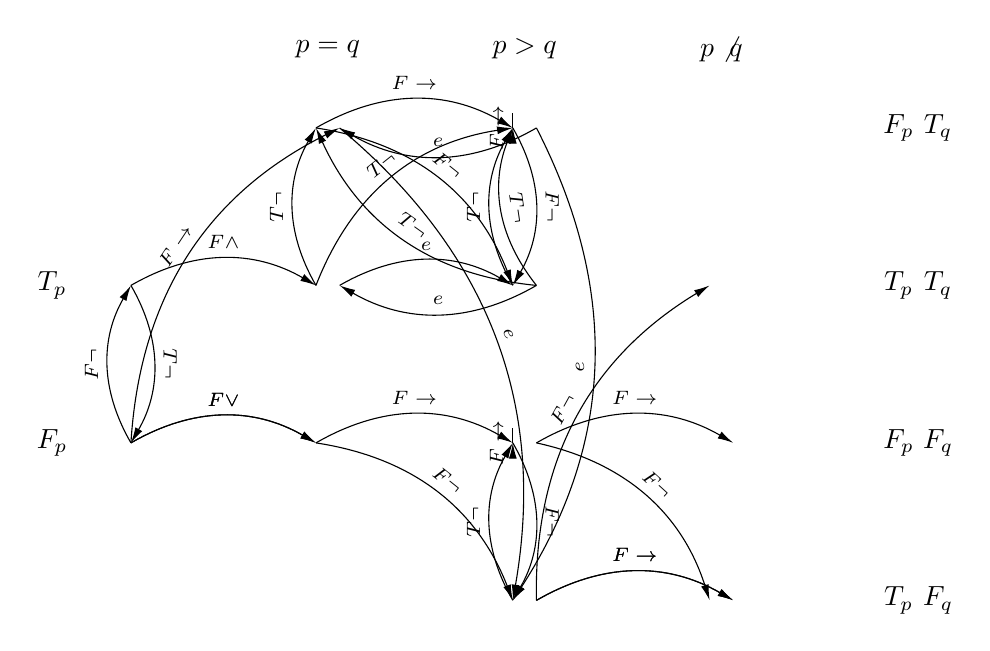
\begin{tikzpicture}

        \node at (\eq, \H) {$p = q$};
        \node at (\gr, \H) {$p > q$};
        \node at (\inc, \H) {$p  \not\lessgtr
        q$ };

        \node at (\Pl, \FT){$F_p$};
        \node at (\Pl, \TT){$T_p$};
        \node at (\Pl, \TF){$T_p$};
        \node at (\Pl, \FF){$F_p$};

        \node at (\Ql, \FT){$T_q$};
        \node at (\Ql, \TT){$T_q$};
        \node at (\Ql, \TF){$F_q$};
        \node at (\Ql, \FF){$F_q$};


        \node at (\ll, \TT){$T_p$};
        \node at (\ll, \FF){$F_p$};

        
        
          

        \draw[bigarrow] (\Peq,\FF) to node[midway, above, sloped] {\scriptsize{$F\neg$}} (\Pgr,\TF);
        \draw[bigarrow] (\Pgr,\FF) to node[midway, above, sloped] {\scriptsize{$F\neg$}} (\Pgr,\TF);
        \draw[bigarrow] (\Qgr,\FF) to node[midway, above, sloped] {\scriptsize{$F\neg$}} (\Pin,\TF);
        \draw[bigarrow] (\Qgr,\TF) to node[midway, above, sloped] {\scriptsize{$F\neg$}} (\Pin,\TT);
        \draw[bigarrow] (\Peq,\FT) to node[midway, above, sloped] {\scriptsize{$F\neg$}} (\Pgr,\TT);
        \draw[bigarrow] (\Pgr,\FT) to node[midway, above, sloped] {\scriptsize{$F\neg$}} (\Pgr,\TT);


        \draw[bigarrow] (\Psol,\FF) to node[midway, above, sloped] {\scriptsize{$F\neg$}} (\Psol,\TT);

 

        \draw[bigarrow] (\Peq,\FF) to node[midway, above, sloped] {\scriptsize{$F\to$}} (\Pgr,\FF);
        \draw[bigarrow] (\Pgr,\FF) to node[midway, above, sloped] {\scriptsize{$F\to$}} (\Pgr,\FF);
        \draw[bigarrow] (\Qgr,\FF) to node[midway, above, sloped] {\scriptsize{$F\to$}} (\Qin,\FF);
        \draw[bigarrow] (\Peq,\FT) to node[midway, above, sloped] {\scriptsize{$F\to$}} (\Pgr,\FT);
        \draw[bigarrow] (\Pgr,\FT) to node[midway, above, sloped] {\scriptsize{$F\to$}} (\Pgr,\FT);
        \draw[bigarrow] (\Qgr,\TF) to node[midway, above, sloped] {\scriptsize{$F\to$}} (\Qin,\TF);
        \draw[bigarrow] (\Qgr,\TF) to node[midway, above, sloped] {\scriptsize{$F\to$}} (\Qin,\TF);

        \draw[bigarrow] (\Psol,\FF) to node[midway, above, sloped] {\scriptsize{$F\to$}} (\Qeq,\FT);

        


        \draw[bigarrow] (\Qeq,\TT) to node[midway, above, sloped] {\scriptsize{$e$}} (\Pgr,\TT);
        \draw[bigarrow] (\Qgr,\TT) to node[midway, above, sloped] {\scriptsize{$e$}} (\Qeq,\TT);
        

        \draw[bigarrow] (\Qgr,\FT) to node[midway, above, sloped] {\scriptsize{$e$}} (\Qeq,\FT);
        \draw[bigarrow] (\Qgr,\FT) to node[midway, above, sloped] {\scriptsize{$e$}} (\Pgr,\TF);
        \draw[bigarrow] (\Qeq,\FT) to node[midway, above, sloped] {\scriptsize{$e$}} (\Pgr,\TF);



        \draw[bigarrow] (\Peq,\TT) to node[midway, above, sloped] {\scriptsize{$T\neg$}} (\Pgr,\FT);
        
        \draw[bigarrow] (\Pgr,\TT) to node[midway, above, sloped] {\scriptsize{$T\neg$}} (\Pgr,\FT);
        \draw[bigarrow] (\Qgr,\TT) to node[midway, above, sloped] {\scriptsize{$T\neg$}} (\Pgr,\FT);


        \draw[bigarrow] (\Peq,\TT) to node[midway, above, sloped] {\scriptsize{$T\neg$}} (\Peq,\FT);
        \draw[bigarrow] (\Qgr,\TT) to node[midway, above, sloped] {\scriptsize{$T\neg$}} (\Peq,\FT);


        \draw[bigarrow] (\Pgr,\TF) to node[midway, above, sloped] {\scriptsize{$T\neg$}} (\Pgr,\FF);

        \draw[bigarrow] (\Psol,\TT) to node[midway, above, sloped] {\scriptsize{$T\neg$}} (\Psol,\FF);


        \draw[bigarrow] (\Psol,\FF) to node[midway, above, sloped] {\scriptsize{$F\lor$}} (\Peq,\FF);

        \draw[bigarrow] (\Psol,\FF) to node[midway, above, sloped] {\scriptsize{$F\lor$}} (\Peq,\FF);


        \draw[bigarrow] (\Psol,\TT) to node[midway, above, sloped] {\scriptsize{$F\land$}} (\Peq,\TT);



    \end{tikzpicture}



}



\def\nnn{
    \begin{tikzpicture}


\node at (\eq, \H) {$p = q$};
\node at (\gr, \H) {$p > q$};
\node at (\inc, \H) {$p  \not\lessgtr
q$ };

\node at (\Pl, \FT){$F_p$};
\node at (\Pl, \TT){$T_p$};
\node at (\Pl, \TF){$T_p$};
\node at (\Pl, \FF){$F_p$};

\node at (\Ql, \FT){$T_q$};
\node at (\Ql, \TT){$T_q$};
\node at (\Ql, \TF){$F_q$};
\node at (\Ql, \FF){$F_q$};


\node at (\ll, \TT){$T_p$};
\node at (\ll, \FF){$F_p$};



  

\draw[bigarrow] (\Peq,\FF) to node[midway, above, sloped] {\scriptsize{$F\neg$}} (\Pgr,\TF);
\draw[bigarrow] (\Pgr,\FF) to node[midway, above, sloped] {\scriptsize{$F\neg$}} (\Pgr,\TF);
\draw[bigarrow] (\Qgr,\FF) to node[midway, above, sloped] {\scriptsize{$F\neg$}} (\Pin,\TF);
\draw[bigarrow] (\Qgr,\TF) to node[midway, above, sloped] {\scriptsize{$F\neg$}} (\Pin,\TT);
\draw[bigarrow] (\Peq,\FT) to node[midway, above, sloped] {\scriptsize{$F\neg$}} (\Pgr,\TT);
\draw[bigarrow] (\Pgr,\FT) to node[midway, above, sloped] {\scriptsize{$F\neg$}} (\Pgr,\TT);


\draw[bigarrow] (\Psol,\FF) to node[midway, above, sloped] {\scriptsize{$F\neg$}} (\Psol,\TT);

\end{tikzpicture}
}
\def\thinnedExampleImageII{
\begin{tikzpicture}

        \node at (\eq, \H) {$p = q$};
        \node at (\gr, \H) {$p > q$};
        \node at (\inc, \H) {$p  \not\lessgtr
        q$ };

        \node at (\Pl, \FT){$F_p$};
        \node at (\Pl, \TT){$T_p$};
        \node at (\Pl, \TF){$T_p$};
        \node at (\Pl, \FF){$F_p$};

        \node at (\Ql, \FT){$T_q$};
        \node at (\Ql, \TT){$T_q$};
        \node at (\Ql, \TF){$F_q$};
        \node at (\Ql, \FF){$F_q$};


        \node at (\ll, \TT){$T_p$};
        \node at (\ll, \FF){$F_p$};

        
        \draw[bigarrow] (\Psol,\FF) to node[midway, above, sloped] {\scriptsize{$F\to$}} (\Qeq,\FT);
        \draw[bigarrow] (\Peq,\FT) to node[midway, above, sloped] {\scriptsize{$F\neg$}} (\Pgr,\TT);

        \draw[bigarrow] (\Pgr,\TT) to node[midway, above, sloped] {\scriptsize{$T\neg$}} (\Pgr,\FT);
          
    
        \draw[bigarrow] (\Qgr,\FT) to node[midway, above, sloped] {\scriptsize{$T\neg$}} (\Qeq,\FT);
    \end{tikzpicture}
}
\def\thinnedExampleImageI
{
        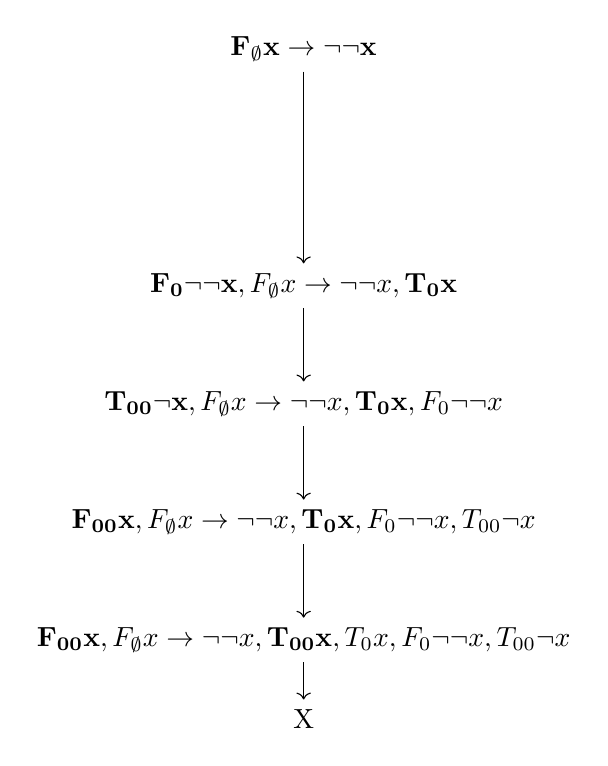
\begin{tikzpicture}
        % Root node
        \node (root) at (0,0) {$\mathbf{F_{\emptyset} x \to \neg \neg x}$};
                
        % Third stage nodes
        \node (n2) at (0,-3) {$\mathbf{F_{0} \neg \neg x}, F_{\emptyset} x \to \neg \neg x, \mathbf{T_{0} x}$};
        \draw[->] (root) -- (n2);
        
        % Fourth stage nodes
        \node (n3) at (0,-4.5) {$ \mathbf{T_{00} \neg x}, F_{\emptyset} x \to \neg \neg x,\mathbf{ T_{0} x},F_{0} \neg \neg x$};
        \draw[->] (n2) -- (n3);
        
        % Fifth stage nodes
        \node (n4) at (0,-6) {$ \mathbf{F_{00}  x}, F_{\emptyset} x \to \neg \neg x, \mathbf{T_{0} x},F_{0} \neg \neg x, T_{00} \neg x$};
        \draw[->] (n3) -- (n4);
        \node (n5) at (0,-7.5) {  $\mathbf{F_{00}x} , F_{\emptyset} x \to \neg \neg x, \mathbf{T_{00} x }    ,T_{0} x,F_{0} \neg \neg x, T_{00} \neg x$};     \draw[->] (n4) -- (n5);


        \node (n6) at (0,-8.5) {X};
        \draw[->] (n5) -- (n6);
    \end{tikzpicture}
}



